
\documentclass[12pt]{mitthesis}

\usepackage{graphicx}
\usepackage{booktabs, chemformula}
\usepackage{titlesec, blindtext, color}
\usepackage{listings}
\usepackage{float}
\usepackage{xcolor} 
\usepackage{array}
\usepackage{color, colortbl}
\usepackage{caption}
\usepackage{amsmath}

\captionsetup{font=footnotesize}

\definecolor{lightgreen}{rgb}{0.82, 0.94, 0.75}
\definecolor{lightorange}{rgb}{0.98, 0.84, 0.65}
\newcolumntype{L}{>{\centering\arraybackslash}m{10cm}}
\newcolumntype{l}{>{\centering\arraybackslash}m{7cm}}
\def\BibTeX{{\rm B\kern-.05em{\sc i\kern-.025em b}\kern-.08em
    T\kern-.1667em\lower.7ex\hbox{E}\kern-.125emX}}

\newcommand*{\Comb}[2]{{}^{#1}C_{#2}}%

\pagestyle{plain}

\usepackage{caption}
\usepackage{subcaption}
\usepackage[a4paper,width=150mm,top=35mm,bottom=35mm,bindingoffset=6mm]{geometry}

\begin{document}
\begin{titlepage}
    \begin{center}
        \vspace*{1cm}
        \large
        \textbf{Methods and Tools for the Analysis of Legacy Software Systems}
            
        \vspace{0.5cm}
        Report 2. Logical dependencies in practice.
            
        \vspace{1.5cm}
            
        \textbf{PhD Student: Adelina Diana Stana}
            
        \vfill
            
        \vspace{0.8cm}
            
        
\includegraphics[width=0.4\textwidth]{Logo-UPT.jpg}

        Department: Calculatoare şi tehnologia informaţiei\\
        PhD Supervisor: Vladimir I. CREŢU\\
            
    \end{center}
\end{titlepage}




\tableofcontents

\pagestyle{plain}

\chapter{Introduction}

In order to obtain logical dependencies, we have to filter the co-changes extracted from the versioning system.
The filtering will increase the confidence that the remaining co-changing pairs are indeed logically coupled.
And also will help to reduce the size of the co-changes extracted. 

We defined 3 methods for filtering the co-changing pairs into logical dependencies. For each method, we analyzed the extracted information from the history of the systems defined in section \ref{sec:dataset}, and we drew the conclusions presented below.

\textbf{Filtering based on the size of commit transactions. }
For this, we filter out each commit transaction that has more files changed than an established threshold.
This type of filtering will significantly reduce the amount of co-changing pairs extracted. Big commit transactions (more than 10 files) are rather related to refactoring of names, spellchecks, or file reformating and not to actual code changes. Less than 10\% of the total commits are commits with more than 10 files. So filtering out every commit that has more than 10 files changed will not impact so much the size of the studied information from the versioning system. After filtering we are remaining with 90\% of commits from which we can extract co-changing pairs.


\textbf{Filtering based on the number of occurrences. }
In this step, we filter out each co-changing pair that does not occur in the versioning system more than an established threshold.
This type of filtering is meant to increase the confidence that the extracted co-changing pairs are logically coupled.
We decided not to go any further with this type of filtering. Mainly because in our experiments, we observed that if we try to go higher with the occurrences threshold, we risk filtering all the existing co-changing pairs for some small systems.
From this filtering method, we concluded that we need to consider the system size and the occurrence trends for each system in particular, rather than setting a "hard" threshold for all the studied systems.

\textbf{Filtering based on connection strength. }
The connection strength is calculated based on the connection factors of both entities that form a co-changing pair. For a co-changing pair formed by entities A and B, the connection factor of entity A with entity B is the percentage from the total commits involving A that contains entity B, the same applies for B with A.
This filter type is meant to establish how important, to one another, the entities that form a co-changing pair are. 
If we filter out all the co-changing pairs that do not update at least half of the time together (factor A and factor B $\geq 50 \%$ ) we remain with a decent quantity of co-changing pairs. And at this point, we can say that the remaining co-changing pairs are logical dependencies.

Based on all the conclusions described above, further in our research, we will use the filter based on commit transaction size ( filter out commits that have more than 10 files changed) and the filter based on connection strength. 



\chapter{Usage of the extracted dependencies}
\section{Data set used}
To extract the key classes based on logical dependencies, we took the same set of data used in another research involving key class detection. The research of I. Sora et al \cite{Finding-key-classes} takes into consideration structural public dependencies that are extracted using static analysis techniques and was performed on the object-oriented systems presented in table \ref{tab:keyclass:overview}.

The requirements for a system to qualify as suited for investigations using logical dependencies are: has to be on GitHub, has to have release tags to identify the version, and also has to have an increased number of commits. 
From the total of 14 object-oriented systems listed in the paper \cite{Finding-key-classes}, 13 of them have repositories in Github \ref{tab:gitfoundsystems}. And from the found repositories we identified only 6 repositories that have the same release tag as the specified version from table \ref{tab:keyclass:overview}. It is important to identify the correct release tag for each repository to limit the commits further analyzed by date. Only commits that were made until the specified release are considered and analyzed.
The commits number found on the remaining 6 repositories varies from 19108 commits for Tomcat Catalina to 149 commits for JHotDraw. In order to have more accurate results, we need a significant number of commits, so we reached the conclusion that only 3 systems can be used for key classes detection using logical dependencies: Apache Ant, Hibernate, and Tomcat Catalina.  From all the systems mentioned in table \ref{tab:keyclass:overview} Apache Ant is the most used and analyzed in other  works \cite{enase19}, \cite{7332515}, \cite{1402122}, \cite{Kamran2016IdentificationOC}.

\begin{table}[H]
\renewcommand{\arraystretch}{1}
\captionsetup{font=scriptsize}
\caption{Analyzed software systems in previous research paper.}
\label{tab:keyclass:overview}
\centering
\scalebox{0.8}{
\begin{tabular}{|c|c|L|c|}
\hline
ID	&	System	&	Description	&	Version	\\
\hline
Sl	&	Apache Ant	&	Java library and command line tool that drive the build processes as targets and extension points depending upon each other	&	1.6.1	\\
S2	&	Argo UML	&	UML modelling tool with support for all UML diagrams.	&	0.9.5	\\
S3	&	GWT Portlets	&	Open source web framework for building GWT (Google Web Toolkit) Applications.	&	0.9.5 beta	\\
S4	&	Hibernate 	&	Persistence framework for Java.	&	5.2.12	\\
S5	&	javaclient	&	Java distributed application for playing with robots	&	2.0.0	\\
S6	&	jEdit	&	Java mature text editor for programmers.	&	5.1.0	\\
S7	&	JGAP	&	Genetic Algorithms and Genetic Programming Java library.	&	3.6.3	\\
S8	&	JHotDraw	&	JHotDraw is a two-dimensional graphics framework for structured drawing editors that is written in Java.	&	6.0b.1	\\
S9	&	JMeter	&	JMeter is a Java application designed to load test functional behavior and measure performance	&	2.0.1	\\
S10	&	Log4j	&	Logging Service	&	2.10.0	\\
S11	&	Mars	&	The Mars Simulation Project is a Java project that models and simulates human settlements on Mars planet	&	3.06.0	\\
S12	&	Maze	&	The Maze-solver project simulates an artificial intelligence algorithm on a maze	&	1.0.0	\\
S13	&	Neuroph	&	Neuroph is a Java neural network framework.	&	2.2.0	\\
S14	&	Tomcat Catalina	&	The Apache Tomcat project is an open-source implementation of JavaServlet and JavaServerPages technologies	&	9.0.4	\\
S15	&	Wro4J	&	The Wro4J is a web resource (JS and CSS) optimizer for Java.	&	1.6.3	\\
\hline
\end{tabular}
}
\end{table}



\begin{table}[H]
\renewcommand{\arraystretch}{1}
\captionsetup{font=scriptsize}
\caption{Found systems and versions of the systems in GitHub. }
\label{tab:gitfoundsystems}
\centering
\scalebox{0.8}{
\begin{tabular}{|c|c|c|c|c|}
\hline
ID	&	System	&	Version	&	Release Tag name	&	Commits number	\\
\hline
\rowcolor{lightgreen}
Sl	&	Apache Ant	&	1.6.1	&	rel/1.6.1	&	6713	\\
S2	&	Argo UML	&	0.9.5	&	not found	&	0	\\
S3	&	GWT Portlets	&	0.9.5 beta	&	not found	&	0	\\
\rowcolor{lightgreen}
S4	&	Hibernate 	&	5.2.12	&	5.2.12	&	6733	\\
S5	&	javaclient	&	2.0.0	&	not found	&	0	\\
S6	&	jEdit	&	5.1.0	&	not found	&	0	\\
S7	&	JGAP	&	3.6.3	&	not found	&	0	\\
S8	&	JHotDraw	&	6.0b.1	&	not found	&	149	\\
S9	&	JMeter	&	2.0.1	&	v2\_1\_1	&	2506	\\
S10	&	Log4j	&	2.10.0	&	v1\_2\_10-recalled	&	634	\\
S11	&	Mars	&	3.06.0	&	not found	&	0	\\
S12	&	Maze	&	1.0.0	&	not found	&	0	\\
S13	&	Neuroph	&	2.2.0	&	not found	&	0	\\
\rowcolor{lightgreen}
S14	&	Tomcat Catalina	&	9.0.4	&	9.0.4	&	19108	\\
S15	&	Wro4J	&	1.6.3	&	v1.6.3	&	2871	\\
\hline
\end{tabular}
}
\end{table}


\section{Identifying key classes using logical dependencies}
\subsection{Definition and previous work}
Zaidman et al \cite{ZaidmanJurnal} were the first to introduce the concept of key classes and it refers to classes that can be found in documents written to provide an architectural overview of the system or an introduction to the system structure. 
Tahvildari and Kontogiannis have a more detailed definition regarding key classes concept: “Usually, the most important concepts of a system are implemented by very few key classes which can be characterized by the specific properties. These classes, which we refer to as key classes, manage many other classes or use them in order to implement their functionality. The key classes are tightly coupled with other parts of the system. Additionally, they tend to be rather complex, since they implement much of the legacy system’s functionality” \cite{Tahvildari2004ImprovingDQ}.
Also, other researchers use a similar concept as the one defined by Zaidman but under different terms like important classes  \cite{Meyer2014IdentifyingIC} or central software classes \cite{CentralClassesSteidl}.


In previous works, the approach for finding key classes is based on ranking the classes with a page ranking algorithm \cite{PagerankENASE}, \cite{enase15}, \cite{Finding-key-classes}, \cite{PagerankSACI} . The page ranking algorithm is a customization of PageRank, the algorithm used to rank web pages \cite{ilprints422}. 
The PageRank algorithm works based on a recommendation system. If one node has a connection with another node, then it recommends the second node. In previous works, connections are established based on structural dependencies extracted from static code analysis. If A has a structural dependency with B, then A recommends B, and also B recommends A. 

\subsection{Attributes for key classes detection}
In order to identify the key classes of an object-oriented system, we have to determine what metrics can be used in order to get a good overview of the system and its most important classes \cite{Ding2016AnIA}, \cite{ZaidmanJurnal}, \cite{PAN2018188} . 
The metrics used in previous research can be grouped into the following categories: 

\begin{itemize}
	\item class size metrics: number of fields (NoF),  number of methods (NoM), global size (Size = NoF+NoM).
	\item class connection metrics, any structural dependency between two classes:
		\begin{itemize}
			\item CONN-IN, the number of distinct classes that use a class;
			\item CONN-OUT, the total number of distinct classes that are used by a class;
			\item CONN-TOTAL, the total number of distinct classes that a class uses or are used by a class (CONN-IN + CONN-OUT).
			\item CONN-IN-W, the total weight of distinct classes that use a class. 
			\item CONN-OUT-W, the total weight of distinct classes that are used by a class. 
			\item CONN-TOTAL-W, the total weight of all connections of the class (CONN-IN-W + CONN-OUT-W) \cite{Finding-key-classes}.
		\end{itemize}
	\item class pagerank values, previous research use pagerank values computed on both directed and undirected, weighted and unweighted graphs:
		\begin{itemize}
			\item PR - value computed on the directed and unweighted graph;
			\item PR-W - value computed on the directed and weighted graph;
			\item PR-U - value computed on the undirected and unweighted graph;
			\item PR-U-W - value computed on the undirected and weighted graph;
			\item PR-U2-W - value computed on the weighted graph with back-recommendations \cite{PagerankENASE}, \cite{enase15}, \cite{Finding-key-classes}, \cite{PagerankSACI}.
		\end{itemize}
\end{itemize}

Because the extracted logical dependencies from the systems are undirected, from the mentioned metrics, we can use the following ones:  CONN-TOTAL, CONN-TOTAL-W, PR-U, PR-U-W and PR-U2-W.

\subsection{Metrics for results evaluation}
\label{sec:evalmetrics}
A classification model is a mapping between expected results and predicted results \cite{ROCIntro}, \cite{ROCBRADLEY19971145}. Both results can be labeled as positive or negative, which leads us to the confusion matrix from figure \ref{fig:confusion}. 

\begin{figure}[h]
\centering
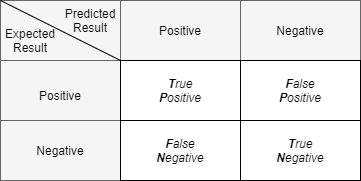
\includegraphics[scale=0.9]{confusion.png}
\caption{Confusion matrix}
\label{fig:confusion}
\centering
\end{figure}

The confusion matrix has the following outcomes:
		\begin{itemize}
			\item \textit{true positive}, if the expected result is positive and the predicted result is also positive.
			\item \textit{false positive}, if the expected result is positive but the predicted result is negative.
			\item \textit{false negative}, if the expected result is negative but the predicted result is positive.
			\item \textit{true negative}, if the expected result is negative and the predicted result is also negative.
		\end{itemize}

The true positive rate of a classifier is calculated as the division between the number of true positive results identified and all the positive results identified:
\[ True\ positive\ rate (TPR)
  = \dfrac{TP}{TP+FN}
\]

The false positive rate of a classifier is calculated as the division between the number of false positive results identified and all the negative results identified:
\[ False\ positive\ rate (FPR)
  = \dfrac{FP}{FP+TN}
\]

To calculate the performance of a classification model, the Receiver Operating Characteristic (ROC) graph can be used. The ROC graph is a two-dimensional graph that has on the X-axis plotted the false positive rate and on the Y-axis the true positive rate. By plotting the true positive rate and the false positive rate at thresholds that vary between a minimum and a maximum possible value we obtain the ROC curve. The area under the ROC curve is called Area Under the Curve (AUC).

In multiple related works, the ROC-AUC metric has been used to evaluate the results for finding key classes of software systems \cite{6676885}, \cite{Finding-key-classes}, \cite{rocclasification}, \cite{7551990}.

For a classifier to be considered good, its ROC-AUC metric value should be as close to 1 as possible, when the value is 1 then the classifier is considered to be perfect.

\subsection{Results obtained by the baseline approach}
\label{sec:previous_measurements}

In the research of I. Sora et al \cite{Finding-key-classes} is used a tool that takes as an input the source code of the system and applies a ranking strategy to rank the classes according to their importance. To differentiate the important classes from the rest of the classes, a TOP threshold for the top classes found is set. The threshold can vary between 20 and 30 classes.

The expected results from the research are based on classes labeled as important classes in the system documentation.
The true positives (TP) are the classes found in the reference solution and also in the top TOP ranked classes. False positives (FP) are the classes that are not in the reference solution but are in the TOP ranked classes.
True Negatives (TN) are classes that are found neither in the reference solution nor in the TOP ranked classes. False Negatives (FN) are classes that are found in the reference solution but not found in the TOP ranked classes.

In table \ref{tab:previousresults} are presented the ROC-AUC values for different attributes computed for the systems Ant, Tomcat Catalina, and Hibernate.

\begin{table}[!h]
\renewcommand{\arraystretch}{1}
\caption{ROC-AUC metric values extracted. }
\label{tab:previousresults}
\centering
\scalebox{0.9}{
\begin{tabular}{|c|ccc|}
\hline
Metrics &	Ant	&	Tomcat Catalina	&	Hibernate	\\
\hline

PR\_U2\_W	&	0.95823	&	0.92341	&	0.95823	\\
PR	&	0.94944	&	0.92670	&	0.94944	\\
PR\_U	&	0.95060	&	0.93220	&	0.95060	\\
CONN\_TOTAL\_W	&	0.94437	&	0.92595	&	0.94437	\\
CONN\_TOTAL	&	0.94630	&	0.93903	&	0.94630	\\

\hline
\end{tabular}
}
\end{table}

\subsection{Measurements using logical dependencies}


To evaluate the results obtained using logical dependencies, we used the same tool used in section X. 
Previously, the tool used only structural dependencies extracted from the source code of the software systems. In this chapter, we intend to add also the logical dependencies from the versioning system to observe if the results could be improved or not.

For this, the logical dependencies used were filtered based on the update percentage of the entities involved. We define a logical dependency as a connection observed via commits in the versioning system between entity A and entity B. The update percentage of entity A with entity B is determined as follows: the percentage from the total commits involving A that contains entity B.

\[ update\ percentage\ for\ A 
  = \dfrac{100 * commits\ involving\ A\ and\ B}{total\ nr\ of\ commits\ involving\ A}
\]

\[ update\ percentage\ for\ B 
  = \dfrac{100 * commits\ involving\ A\ and\ B}{total\ nr\ of\ commits\ involving\ B}
\]

We calculated the update percentage for each side of the connection (LD) and filtered the connections found based on it. The rule set is that both entities had to have an update percentage with each other greater than the threshold value.
In tables \ref{tab:measurementscombined:ant}, \ref{tab:measurementscombined:tomcat}, and \ref{tab:measurementscombined:hibernate}, we introduced the logical dependencies among structural dependencies. We started with logical dependencies that have a percentage of update grater then 10\%, which means that in at least 10\% of the commits involving A or B, A and B update together. Then we increased the threshold value by 10 until we remained only with entities that update in all the commits together.

As for the new results obtained, in tables \ref{tab:measurementscombined:ant}, \ref{tab:measurementscombined:tomcat}, and \ref{tab:measurementscombined:hibernate}, highlighted with orange, are the values that are close to the previously registered values but did not surpass them. Highlighted with green are values that are better than the previously registered values.

\begin{table}[!h]
\renewcommand{\arraystretch}{1}
\caption{Measurements for Ant using structural and logical dependencies combined}
\label{tab:measurementscombined:ant}
\centering
\scalebox{0.8}{
\begin{tabular}{|c|cccccccccc|c|}
\hline
Metrics &	$\geq10\%$	&	$\geq20\%$		&	$\geq30\%$		&	$\geq40\%$		&	$\geq50\%$		&	$\geq60\%$		&	$\geq70\%$		&	$\geq80\%$		&	$\geq90\%$		&	$\geq100\%$		&	Previous \\
\hline

PR\_U2\_W	&	0.924	&	0.925	&	0.926	&	0.927	&	0.927	&	0.927	&	\cellcolor{lightgreen}0.929	&	0.928	&	0.928	&	0.928	&	0.929	\\
PR	&	0.914	&	0.854	&	0.851	&	0.866	&	0.876	&	0.882	&	\cellcolor{lightgreen}0.887	&	0.854	&	0.852	&	0.852	&	0.855	\\
PR\_U	&	0.910	&	0.930	&	0.933	&	0.933	&	0.935	&	0.934	&	\cellcolor{lightgreen}0.939	&	0.933	&	0.933	&	0.933	&	0.933	\\
CONN\_T\_W	&	0.924	&	0.928	&	0.931	&	0.932	&	0.933	&	0.934	&	\cellcolor{lightgreen}0.936	&	0.934	&	0.934	&	0.934	&	0.934	\\
CONN\_T	&	0.840	&	0.886	&	0.904	&	0.909	&	0.915	&	0.923	&	0.932	&	0.935	&	\cellcolor{lightorange}0.936	&	0.936	&	0.942	\\

\hline
\end{tabular}
}
\end{table}


\begin{table}[!h]
\renewcommand{\arraystretch}{1}
\caption{Measurements for Tomcat using structural and logical dependencies combined}
\label{tab:measurementscombined:tomcat}
\centering
\scalebox{0.8}{
\begin{tabular}{|c|cccccccccc|c|}
\hline
Metrics &	$\geq10\%$	&	$\geq20\%$		&	$\geq30\%$		&	$\geq40\%$		&	$\geq50\%$		&	$\geq60\%$		&	$\geq70\%$		&	$\geq80\%$		&	$\geq90\%$		&	$\geq100\%$		&	Previous \\
\hline

PR\_U2\_W	&	0.912	&	0.915	&	0.922	&	0.923	&	\cellcolor{lightgreen}0.924	&	0.924	&	0.923	&	0.924	&	0.924	&	0.924	&	0.923	\\
PR	&	0.808	&	0.785	&	0.812	&	0.839	&	0.844	&	0.851	&	0.853	&	\cellcolor{lightorange}0.857	&	0.857	&	0.857	&	0.927	\\
PR\_U	&	0.912	&	0.920	&	0.931	&	0.932	&	\cellcolor{lightgreen}0.933	&	0.933	&	0.933	&	0.932	&	0.932	&	0.932	&	0.932	\\
CONN\_T\_W	&	0.918	&	0.921	&	0.924	&	\cellcolor{lightgreen}0.926	&	0.926	&	0.926	&	0.926	&	0.926	&	0.926	&	0.926	&	0.926	\\
CONN\_T	&	0.877	&	0.913	&	0.932	&	0.937	&	0.937	&	\cellcolor{lightorange}0.938	&	0.938	&	0.938	&	0.938	&	0.938	&	0.939	\\					

\hline
\end{tabular}
}
\end{table}


\begin{table}[!h]
\renewcommand{\arraystretch}{1}
\caption{Measurements for Hibernate using structural and logical dependencies combined}
\label{tab:measurementscombined:hibernate}
\centering
\scalebox{0.8}{
\begin{tabular}{|c|cccccccccc|c|}
\hline
Metrics &	$\geq10\%$	&	$\geq20\%$		&	$\geq30\%$		&	$\geq40\%$		&	$\geq50\%$		&	$\geq60\%$		&	$\geq70\%$		&	$\geq80\%$		&	$\geq90\%$		&	$\geq100\%$		&	Previous \\
\hline

PR\_U2\_W	&	0.955	&	0.957	&	\cellcolor{lightorange}0.958	&	0.958	&	0.958	&	0.958	&	0.958	&	0.958	&	0.958	&	0.958	&	0.958	\\
PR	&	0.931	&	0.930	&	0.936	&	0.940	&	0.940	&	\cellcolor{lightorange}0.946	&	0.946	&	0.946	&	0.946	&	0.946	&	0.949	\\
PR\_U	&	0.942	&	0.946	&	0.948	&	0.949	&	0.949	&	\cellcolor{lightorange}0.950	&	0.950	&	0.950	&	0.950	&	0.950	&	0.951	\\
CONN\_T\_W	&	0.939	&	0.942	&	0.943	&	\cellcolor{lightgreen}0.944	&	0.944	&	0.944	&	0.945	&	0.945	&	0.945	&	0.945	&	0.944	\\
CONN\_T	&	0.925	&	0.933	&	0.938	&	0.940	&	0.941	&	\cellcolor{lightorange}0.944	&	0.944	&	0.944	&	0.944	&	0.944	&	0.946	\\

\hline
\end{tabular}
}
\end{table}


%%%%%%%%%%%%%%%%%%%%%%%%%%%%%%%%%%%%%%%%

In tables \ref{tab:measurementshistory:ant}, \ref{tab:measurementshistory:tomcat}, and \ref{tab:measurementshistory:hibernate}, we only used logical dependencies. The measurements obtained by using only logical dependencies are not as good as using logical and structural dependencies combined or using only structural dependencies.
As mentioned in section \ref{sec:evalmetrics}, a classifier is good if it has the ROC-AUC value as close to 1 as possible. Our classifier identifies the key classes of a software system, classes that are also called central classes. 
The central classes may have a better design than the rest of the classes, which means that are less prone to change. If the key classes are less prone to change, this implies that the number of dependencies extracted from the versioning system can be less than for other classes. 

\begin{table}[!h]
\renewcommand{\arraystretch}{1}
\caption{Measurements for Ant using only logical dependencies}
\label{tab:measurementshistory:ant}
\centering
\scalebox{0.8}{
\begin{tabular}{|c|cccccccccc|c|}
\hline
Metrics &	$\geq10\%$	&	$\geq20\%$		&	$\geq30\%$		&	$\geq40\%$		&	$\geq50\%$		&	$\geq60\%$		&	$\geq70\%$		&	$\geq80\%$		&	$\geq90\%$		&	$\geq100\%$		&	Previous \\
\hline

PR\_U2\_W	&	0.655	&	0.611	&	0.650	&	0.645	&	0.729	&	0.797	&	0.855	&	0.882	&	0\cellcolor{lightorange}.865	&	0.865	&	0.929	\\
PR	&	0.655	&	0.611	&	0.650	&	0.645	&	0.729	&	0.797	&	0.855	&	\cellcolor{lightorange}0.882	&	0.865	&	0.865	&	0.855	\\
PR\_U	&	0.655	&	0.611	&	0.650	&	0.645	&	0.729	&	0.797	&	0.855	&	\cellcolor{lightorange}0.882	&	0.865	&	0.865	&	0.933	\\
CONN\_T\_W	&	0.646	&	0.523	&	0.617	&	0.657	&	0.722	&	0.785	&	0.845	&	\cellcolor{lightorange}0.878	&	0.865	&	0.865	&	0.934	\\
CONN\_T	&	0.646	&	0.523	&	0.617	&	0.657	&	0.722	&	0.785	&	0.845	&	\cellcolor{lightorange}0.878	&	0.865	&	0.865	&	0.942	\\

\hline
\end{tabular}
}
\end{table}


\begin{table}[!h]
\renewcommand{\arraystretch}{1}
\caption{Measurements for Tomcat using only logical dependencies}
\label{tab:measurementshistory:tomcat}
\centering
\scalebox{0.8}{
\begin{tabular}{|c|cccccccccc|c|}
\hline
Metrics &	$\geq10\%$	&	$\geq20\%$		&	$\geq30\%$		&	$\geq40\%$		&	$\geq50\%$		&	$\geq60\%$		&	$\geq70\%$		&	$\geq80\%$		&	$\geq90\%$		&	$\geq100\%$		&	Previous \\
\hline

PR\_U2\_W	&	0.702	&	0.627	&	0.627	&	0.712	&	0.741	&	0.775	&	0.786	&	\cellcolor{lightorange}0.796	&	0.796	&	0.796	&	0.923	\\
PR	&	0.675	&	0.617	&	0.627	&	0.712	&	0.741	&	0.775	&	0.786	&	\cellcolor{lightorange}0.796	&	0.796	&	0.796	&	0.927	\\
PR\_U	&	0.675	&	0.618	&	0.627	&	0.712	&	0.741	&	0.775	&	0.786	&	\cellcolor{lightorange}0.796	&	0.796	&	0.796	&	0.932	\\
CONN\_T\_W	&	0.676	&	0.597	&	0.624	&	0.712	&	0.741	&	0.775	&	0.786	&	\cellcolor{lightorange}0.796	&	0.796	&	0.796	&	0.926	\\
CONN\_T	&	0.638	&	0.585	&	0.624	&	0.712	&	0.741	&	0.775	&	0.786	&	\cellcolor{lightorange}0.796	&	0.796	&	0.796	&	0.939	\\
				
\hline
\end{tabular}
}
\end{table}


\begin{table}[!h]
\renewcommand{\arraystretch}{1}
\caption{Measurements for Hibernate using only logical dependencies}
\label{tab:measurementshistory:hibernate}
\centering
\scalebox{0.8}{
\begin{tabular}{|c|cccccccccc|c|}
\hline
Metrics &	$\geq10\%$	&	$\geq20\%$		&	$\geq30\%$		&	$\geq40\%$		&	$\geq50\%$		&	$\geq60\%$		&	$\geq70\%$		&	$\geq80\%$		&	$\geq90\%$		&	$\geq100\%$		&	Previous \\
\hline

PR\_U2\_W	&	0.651	&	0.596	&	0.597	&	0.616	&	0.619	&	0.644	&	0.649	&	\cellcolor{lightorange}0.650	&	0.650	&	0.650	&	0.958	\\
PR	&	0.641	&	0.594	&	0.597	&	0.616	&	0.619	&	0.644	&	0.649	&	\cellcolor{lightorange}0.650	&	0.650	&	0.650	&	0.949	\\
PR\_U	&	0.641	&	0.595	&	0.597	&	0.616	&	0.619	&	0.644	&	0.649	&	\cellcolor{lightorange}0.650	&	0.650	&	0.650	&	0.951	\\
CONN\_T\_W	&	0.652	&	0.591	&	0.597	&	0.616	&	0.619	&	0.644	&	0.649	&	\cellcolor{lightorange}0.650	&	0.650	&	0.650	&	0.944	\\
CONN\_T	&	0.649	&	0.591	&	0.597	&	0.616	&	0.619	&	0.644	&	0.649	&	\cellcolor{lightorange}0.650	&	0.650	&	0.650	&	0.946	\\

\hline
\end{tabular}
}
\end{table}


\section{Comparison of the extracted data with fan-in and fan-out metric}

Fan-in and fan-out are coupling metrics. The fan-in of entity A is the total number of modules that call functions of A. The fan-out of A is the total number of entities called by A \cite{5507329}.
Related to fan-in and fan-out we have extracted CONN\_IN and CONN\_OUT. 

In tables \ref{tab:measurementsfan:ant}, \ref{tab:measurementsfan:catalina}, and \ref{tab:measurementsfan:hibernate} we can find the metrics detalis for each documented key class.

\begin{table}[!h]
\renewcommand{\arraystretch}{1}
\caption{Measurements for Ant key classes}
\label{tab:measurementsfan:ant}
\centering
\scalebox{0.8}{
\begin{tabular}{|c|ccccc|}
\hline
Nr.	&	Classname	&	CONN\_IN	&	CONN\_OUT	&	CONN\_TOTAL	&	LD \\
\hline
1	&	Project	&	191	&	191	&	214	&	157	\\
2	&	Target	&	28	&	28	&	34	&	78	\\
3	&	UnknownElement	&	17	&	17	&	30	&	90	\\
4	&	RuntimeConfigurable	&	11	&	11	&	19	&	118	\\
5	&	IntrospectionHelper	&	18	&	18	&	42	&	143	\\
6	&	Main	&	1	&	1	&	14	&	82	\\
7	&	TaskContainer	&	11	&	11	&	12	&	21	\\
8	&	ProjectHelper2\$ElementHandler	&	1	&	1	&	13	&	30	\\
9	&	Task	&	110	&	110	&	117	&	88	\\
10	&	ProjectHelper	&	16	&	16	&	24	&	101	\\
\hline
\end{tabular}
}
\end{table}




\begin{table}[!h]
\renewcommand{\arraystretch}{1}
\caption{Measurements for Tomcat Catalina key classes.}
\label{tab:measurementsfan:catalina}
\centering
\scalebox{0.8}{
\begin{tabular}{|c|ccccc|}
\hline
Nr.	&	Classname	&	CONN\_IN	&	CONN\_OUT	&	CONN\_TOTAL	&	LD \\
\hline
1	&	Context	&	74	&	8	&	82	&	126	\\
2	&	Request	&	48	&	28	&	76	&	215	\\
3	&	Container	&	51	&	8	&	59	&	64	\\
4	&	Response	&	38	&	12	&	50	&	90	\\
5	&	StandardContext	&	11	&	38	&	49	&	216	\\
6	&	Connector	&	23	&	9	&	32	&	89	\\
7	&	Session	&	29	&	2	&	31	&	28	\\
8	&	Valve	&	29	&	2	&	31	&	19	\\
9	&	Wrapper	&	29	&	1	&	30	&	36	\\
10	&	Manager	&	25	&	3	&	28	&	31	\\
11	&	Host	&	26	&	1	&	27	&	44	\\
12	&	Service	&	20	&	6	&	26	&	51	\\
13	&	Engine	&	23	&	2	&	25	&	1	\\
14	&	Realm	&	18	&	6	&	24	&	21	\\
15	&	CoyoteAdapter	&	1	&	22	&	23	&	140	\\
16	&	StandardHost	&	8	&	15	&	23	&	88	\\
17	&	LifecycleListener	&	21	&	1	&	22	&	3	\\
18	&    StandardEngine	&	2	&	19	&	21	&	57	\\
19	&	Pipeline	&	19	&	2	&	21	&	20	\\
20	&	Server	&	16	&	4	&	20	&	49	\\
21	&	HostConfig	&	3	&	15	&	18	&	79	\\
22	&	StandardWrapper	&	5	&	13	&	18	&	92	\\
23	&	StandardService	&	3	&	12	&	15	&	81	\\
24	&	Catalina	&	2	&	13	&	15	&	94	\\
25	&	Loader	&	14	&	1	&	15	&	18	\\
26	&	StandardServer	&	2	&	12	&	14	&	94	\\
27	&	StandardPipeline	&	1	&	10	&	11	&	62	\\
28	&	Bootstrap	&	3	&	3	&	6	&	41	\\	
\hline
\end{tabular}
}
\end{table}

\begin{table}[!h]
\renewcommand{\arraystretch}{1}
\caption{Measurements for Hibernate key classes.}
\label{tab:measurementsfan:hibernate}
\centering
\scalebox{0.8}{
\begin{tabular}{|c|ccccc|}
\hline
Nr.	&	Classname	&	CONN\_IN	&	CONN\_OUT	&	CONN\_TOTAL	&	LD \\
\hline
1	&	SessionFactoryImplementor	&	438	&	43	&	481	&	51	\\
2	&	Type	&	444	&	5	&	449	&	0	\\
3	&	Table	&	89	&	29	&	118	&	82	\\
4	&	SessionImplementor	&	52	&	12	&	64	&	14	\\
5	&	Criteria	&	45	&	12	&	57	&	15	\\
6	&	Column	&	46	&	10	&	56	&	20	\\
7	&	Session	&	31	&	21	&	52	&	52	\\
8	&	Query	&	12	&	28	&	40	&	0	\\
9	&	Configuration	&	1	&	38	&	39	&	115	\\
10	&	SessionFactory	&	24	&	12	&	36	&	33	\\
11	&	Criterion	&	30	&	3	&	33	&	0	\\
12	&	Projection	&	11	&	3	&	14	&	0	\\
13	&	ConnectionProvider	&	12	&	2	&	14	&	0	\\
14	&	Transaction	&	11	&	1	&	12	&	0	\\
				
\hline
\end{tabular}
}
\end{table}

%%%%%%%%%%%%%%%%%%%%%%%%%%%%%%%%%%%%%%%%%%%%%%%%%%%%%%%%%%%%%%%%%%%%%%%%%%%%%

In tables \ref{tab:measurementstop:ant}, \ref{tab:measurementstop:catalina}, and \ref{tab:measurementstop:hibernate} we can find the top 10 'best ranked' logical dependencies. As we can observe, the entities have only few structural connections.


Highlighed with orange are the key classes found in top 10.
To be continued....

\begin{table}[!h]
\renewcommand{\arraystretch}{1}
\caption{Top 10 measurements for Ant. }
\label{tab:measurementstop:ant}
\centering
\scalebox{0.8}{
\begin{tabular}{|c|ccccc|}
\hline
Nr.	&	Classname	&	CONN\_IN	&	CONN\_OUT	&	CONN\_TOTAL	&	LD \\
\hline
1	&	\cellcolor{lightorange}Project	&	191	&	23	&	214	&	157	\\
2	&	Project\$AntRefTable	&	1	&	2	&	3	&	157	\\
3	&	Path	&	39	&	13	&	52	&	147	\\
4	&	Path\$PathElement	&	3	&	2	&	5	&	147	\\
5	&	\cellcolor{lightorange}IntrospectionHelper	&	18	&	24	&	42	&	143	\\
6	&	IntrospectionHelper\$AttributeSetter	&	8	&	1	&	9	&	143	\\
7	&	IntrospectionHelper\$Creator	&	3	&	5	&	8	&	143	\\
8	&	IntrospectionHelper\$NestedCreator	&	7	&	1	&	8	&	143	\\
9	&	Ant	&	2	&	15	&	17	&	136	\\
10	&	Ant\$Reference	&	3	&	1	&	4	&	136	\\
\hline
\end{tabular}
}
\end{table}

\begin{table}[!h]
\renewcommand{\arraystretch}{1}
\caption{Top 10 measurements for Tomcat Catalina. }
\label{tab:measurementstop:catalina}
\centering
\scalebox{0.8}{
\begin{tabular}{|c|ccccc|}
\hline
Nr.	&	Classname	&	CONN\_IN	&	CONN\_OUT	&	CONN\_TOTAL	&	LD \\
\hline
1	&	\cellcolor{lightorange}StandardContext	&	11	&	38	&	49	&	216	\\
2	&	StandardContext\$ContextFilterMaps	&	0	&	0	&	0	&	216	\\
3	&	StandardContext\$NoPluggabilityServletContext	&	0	&	0	&	0	&	216	\\
4	&	\cellcolor{lightorange}Request	&	48	&	28	&	76	&	215	\\
5	&	Request\$SpecialAttributeAdapter	&	0	&	0	&	0	&	215	\\
6	&	ApplicationContext	&	3	&	22	&	25	&	158	\\
7	&	ApplicationContext\$DispatchData	&	0	&	0	&	0	&	158	\\
8	&	ContextConfig	&	3	&	26	&	29	&	143	\\
9	&	ContextConfig\$DefaultWebXmlCacheEntry	&	0	&	0	&	0	&	143	\\
10	&	ContextConfig\$JavaClassCacheEntry	&	0	&	0	&	0	&	143	\\
\hline
\end{tabular}
}
\end{table}


\begin{table}[!h]
\renewcommand{\arraystretch}{1}
\caption{Top 10 measurements for Hibernate. }
\label{tab:measurementstop:hibernate}
\centering
\scalebox{0.8}{
\begin{tabular}{|c|ccccc|}
\hline
Nr.	&	Classname	&	CONN\_IN	&	CONN\_OUT	&	CONN\_TOTAL	&	LD \\
\hline
1	&	AvailableSettings	&	1	&	0	&	1	&	205	\\
2	&	AbstractEntityPersister	&	9	&	143	&	152	&	190	\\
3	&	AbstractEntityPersister\$CacheEntryHelper	&	0	&	0	&	0	&	190	\\
4	&	AbstractEntityPersister\$InclusionChecker	&	0	&	0	&	0	&	190	\\
5	&	AbstractEntityPersister\$NoopCacheEntryHelper	&	0	&	0	&	0	&	190	\\
6	&	AbstractEntityPersister\$ReferenceCacheEntryHelper	&	0	&	0	&	0	&	190	\\
7	&	AbstractEntityPersister\$StandardCacheEntryHelper	&	0	&	0	&	0	&	190	\\
8	&	AbstractEntityPersister\$StructuredCacheEntryHelper	&	0	&	0	&	0	&	190	\\
9	&	Dialect	&	265	&	104	&	369	&	176	\\
10	&	SessionFactoryImpl\$SessionBuilderImpl	&	1	&	25	&	26	&	167	\\
\hline
\end{tabular}
}
\end{table}

\chapter{Conclusions}

 %%%%%%%%%%%%%%%%%%%%%%%%%%%%%%%%%%%%%%%%%%%%%%%%%%%%%%%%%%%%%%%%%%%%%%%%%%%%%%%%


\bibliographystyle{plain}
\bibliography{logicaldepd}
\end{document}

